\section{Experimental evaluations}
\label{sec:experimental_evaluation}

Here, we show that, despite its simplicity, PATH provides very high quality solutions with a significantly small running time w.r.t. FORTIFY, both in synthetic and real-world instances. 

\subsection{Testbed}
To test PATH, we generate and solve instances that are similar to the ones tested in~\cite{mc2016preventing}, that we know can be solved also by FORTIFY in a reasonable amount of time. Our testbed includes the following graphs:

%Then, we test the scalability and performance of SHARD increaing the dimension of the graph, i.e., the number of nodes and edges, the budget available to the Defender for building its team and the pool of possible resources that can be chosen. We show that SHARD can solve instances significantly larger than FORTIFY along those three dimensions and, when the optimal value requires too much computational effort to be computed, we compare the quality of our solution directly with the value of the most valuable target. In other words, we compare SHARD with a perfect protection of the whole environment. Our testbed includes the following graphs:
%Here, we show that, despite its simplicity, Algorithm~\ref{alg:approximation} provides very high quality solutions with a significantly small runningtime w.r.t. FORTIFY, both in synthetic and real-world instances. Thus, we generate and solve the same instances tested in~\cite{mc2016preventing}, that we know can be solved also by FORTIFY in a reasonable amount of time. Then, we test the scalability and performance of SHARD increaing the dimension of the graph, i.e., the number of nodes and edges, the budget available to the Defender for building its team and the pool of possible resources that can be chosen. We show that SHARD can solve instances significantly larger than FORTIFY along those three dimensions and, when the optimal value requires too much computational effort to be computed, we compare the quality of our solution directly with the value of the most valuable target. In other words, we compare SHARD with a perfect protection of the whole environment. Our testbed includes the following graphs:
\begin{itemize}
\item Geometric graphs: they provide a good approximation of real road networks~\cite{eppstein2008studying}, allowing us to model the networks of villages and rivers in forest regions. $n$ nodes, which include some source nodes $s$ and some targets $t$, are distributed randomly in a plane and are connected based on their distance $r$, which determines the density of the graph. We label such graphs as $R_{n,s,t,r}$.
\item Grid graphs $G_{w,h,s,t}$: they consist of a grid with width $w$, height $h$, $s$ source nodes, $t$ targets and nearest neighbor connections between nodes. We also define starting and ending points for $\mathcal{A}$, with sources located at one end of the graph and targets at the other.
\item Madagascar graph: this graph is a network built from GIS data of at-risk forest areas in Madagascar.
\end{itemize}

Algorithms are implemented in Java 6u45 and are executed on a Linux cluster with HP-SL250, 2.4 GHz, dual-processor machines. In the figures, the budget varies on the $x$-axis while on the $y$-axis we report either the utility ratios or the time ratios of PATH, which adopts the various heuristics, w.r.t. FORTIFY.

\subsection{Synthetic instances}\label{sec:old_synth_comp}
%We evaluate the performance of PATH on the same instances analyzed in~\cite{mc2016preventing}. 
In this section, we focus on synthetic experiments. In particular, we analyze grid graphs $G_{4,4,4,4}$ and geometric graphs $R_{25,4,4,0.1}$. The resources have the following features $L = \{2,2,5,3,3,6\}, P = \{0.7,0.9,0.7,0.6,0.6,0.6\}, b = \{5,8,10,5,8,10\}$ and the Defender can spend budget $B \in \{10, 15, 20, 25\}$. Proceeding this way, on one side we are sure that FORTIFY can solve the problem in a reasonable amount of time, on the other we are not \textit{saturating} the problem, i.e., the budget is not high enough to allow the construction of a team that covers perfectly each target.

\begin{figure}[!htbp]
\centering
\subfigure[Utility ratios]
  {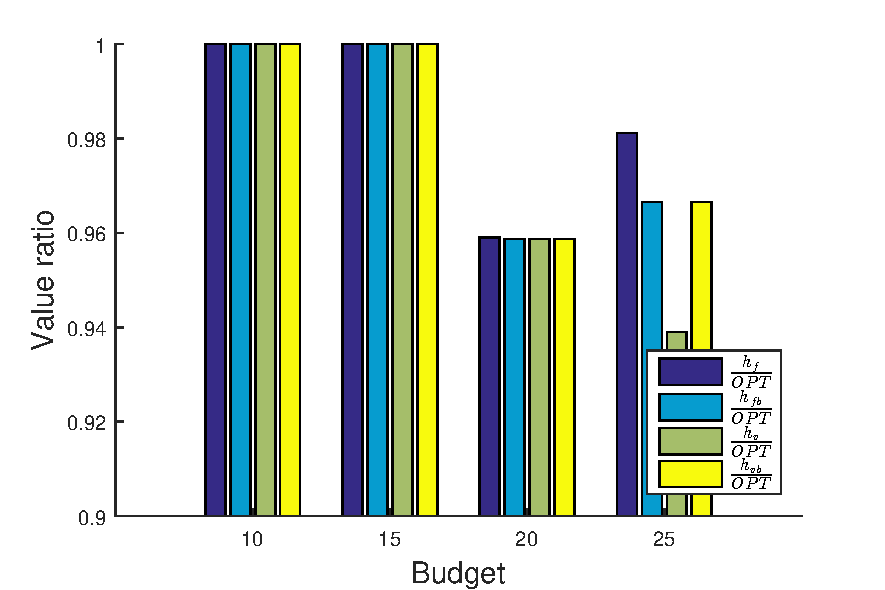
\includegraphics[width=0.48\textwidth]{images/bars_grid_value_ratio}\label{fig:previous_grid_utility}}
\subfigure[Time ratios]
 {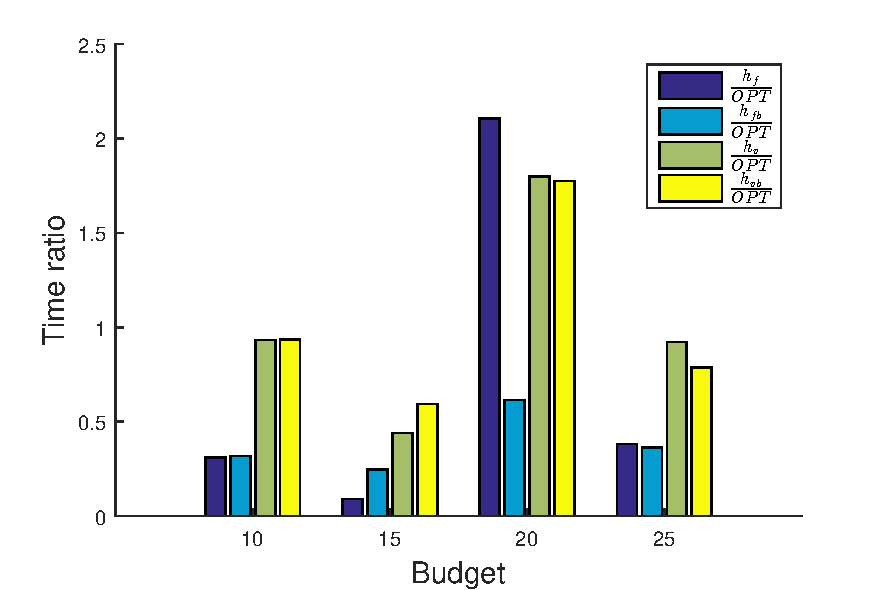
\includegraphics[width=0.48\textwidth]{images/bars_grid_time_ratio}\label{fig:previous_grid_time}}
\caption{Utility and time ratios of PATH w.r.t. FORTIFY on grid graphs.}\label{fig:previous_grid}
\end{figure}

\begin{figure}[!htbp]
\centering
\subfigure[Utility ratios]
  {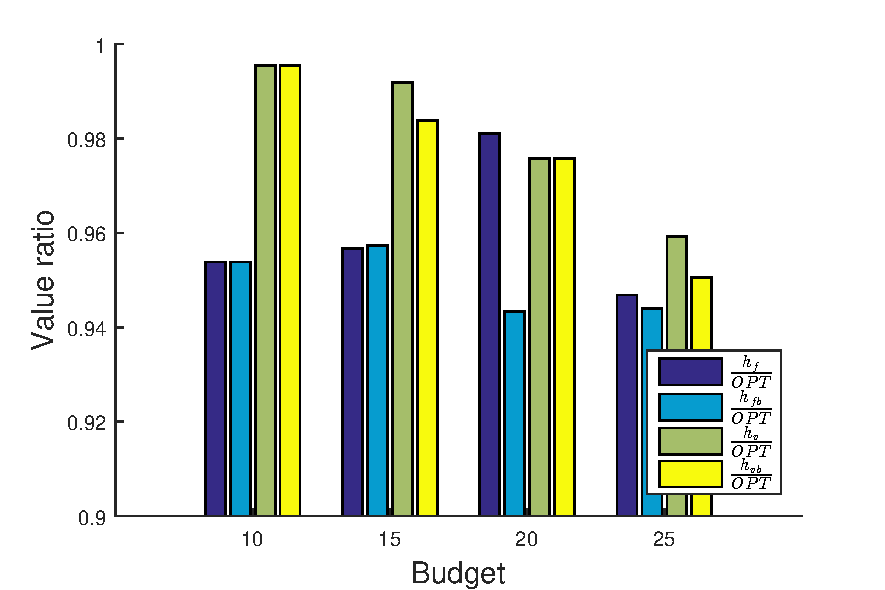
\includegraphics[width=0.46\textwidth]{images/bars_random_value_ratio}\label{fig:previous_random_utility}}
\subfigure[Time ratios]
 {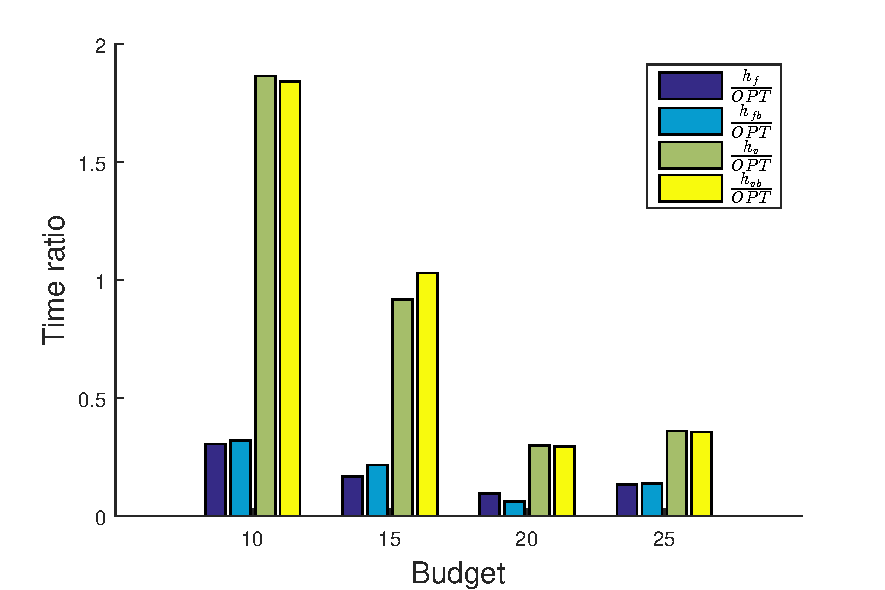
\includegraphics[width=0.46\textwidth]{images/bars_random_time_ratio}\label{fig:previous_random_time}}
\caption{Utility and time ratios of PATH w.r.t. FORTIFY on random graphs.}\label{fig:previous_random}
\end{figure}

\textit{Grid graphs}. Figure~\ref{fig:previous_grid_utility} shows that for low values of the budget, all the heuristics select the same team, getting an approximation ratio higher than 95\% with a budget of 20. If we look at a budget equal to 25, we observe that only $h_v$ is performing worse than the others, but the value is still higher than 94\% of the optimal solution.

Figure~\ref{fig:previous_grid_time} shows the time required by the heuristics w.r.t. the time needed to solve the problem exactly. As we expected, $h_f, h_{fb}$ are faster than $h_v, h_{vb}$, which need to solve the problem also for each single resource. In general, the time required by PATH depends mainly on the time required to solve the exact problem with the team chosen by the heuristic. Thus, depending on the resources the team is composed of and the ways in which such resources can be allocated on the graph, the required time may vary significantly. This explains the (apparently) unusual trends of the time ratios.

%if we include the budget to evaluate the resources, then the resources have the same effectiveness both if we consider their features or the actual value computed solving the problem with such resources as teams of cardinality 1: both methods return an approximation ratio higher than 0.95 as the budget increases. On the other side, if we do not take into account the budget, there is a difference, which is very small: in fact, if we consider the features of the resources, we can provide a utility approximation ratio of 95\% against a worst case of slightly less than 94\% when the budget is equal to 20.

\textit{Random graphs}. Looking at Figure~\ref{fig:previous_random}, we observe that there is a clear difference both in terms of quality solution and computational time for the two main approaches of the heuristics, namely, taking into account the features of the resources or their actual values. Specifically, Figure~\ref{fig:previous_random_utility} shows that, even though the utility ratios are all above 94\%, if we consider the resources according to the utility obtained solving the exact problem, the value computed by the team they chose is higher than the corresponding ones chosen by the other two heuristics. Moreover, the budget does not seem to be a discriminating feature, being $h_f, h_{fb}$ close to each other, and the same holds for $h_v, h_{vb}$. We notice that $h_v$ returns a value equal to 96\% even with a budget of 25.

We focus now on Figure~\ref{fig:previous_random_time}: also in this case, we notice that the budget is not a distinctive feature. Indeed, the times required by $h_f, h_{fb}$ are similar and the same holds for $h_v, h_{vb}$. We observe that for low budgets the time required by the heuristics that adopts the exact values are very high. This is due to the \textit{fixed cost} such heuristics have to pay, namely solving the problem exactly for each resource and then for the chosen team. As the budget increases, FORTIFY requires more and more time because the number of teams to be exactly evaluated grows quickly: our heuristics do not have this issue and consequently, as the budget increases, their time decreases w.r.t. the time required by FORTIFY.


%\subsection{Increasing the size of the graph}\label{sec:synth_size_comp}
%We start increasing the size of the graphs. Specifically, we test SHARD and FORTIFY on the following graphs:
%\begin{itemize}
%\item $R_{25,4,4,r}$ and $r \in \{0.2,0.3\}$;
%\item $R_{30,5,5,r}$ and $r \in \{0.1,0.2,0.3\}$;
%\item $R_{35,6,6,r}$ and $r \in \{0.1,0.2,0.3\}$;
%\item $G_{5,5,s,t}$ with $(s,t) \in \{(2,8),(5,5),(8,2)\}$
%\item $G_{6,6,s,t}$ with $(s,t) \in \{(4,10),(6,6),(10,4)\}$ 
%\end{itemize}
%We employ two sets of resources: $L_1 = \{2,4,5,3,5,6\}, P_1 = \{0.8,0.8,0.8,0.6,0.6,0.6\}, b_1 = \{5,8,10,5,8,10\}$ and $L_2 = \{1,2,3,4,4,6\}, P_2 = \{0.5,0.8,0.7,0.6,0.8,0.9\}, b_2 = \{2,5,8,7,10,12\}$. (We observe that the budget and the number of resources are the same of the previous section).
%
%\subsection{Increasing the budget and the pool of resources}\label{sec:synth_res_comp}
%Here we increase the pool of resources available to $\mathcal{D}$. Specifically, $L = \{1,2,3,4,4,5,5,6,6\}, P = \{0.5,0.8,0.6,0.6,0.7,0.6,0.8,0.6,0.9\}, b = \{2,5,5,7,8,8,10,10,12\}$. We also increase the budget that the Defender can invest to build her team. The graphs we consider are the same of Sec.~\ref{sec:old_synth_comp}.
%
%\subsection{Increasing size, budget and pool of resources}
%Now, we increase our instances along all the three dimensions, considering graphs from Sec.~\ref{sec:synth_size_comp} and resources and budget from Sec.~\ref{sec:synth_res_comp}.

\subsection{Real-world comparison: protecting the Madagascar forests}
We present the following model, which was built working closely with domain experts from NGOs.

\textit{Graph}. We used the road and river networks used by the patrolling officers, as well as the known routes taken by groups of illegal loggers, to build the nodes and edges of our network. Edges correspond to distances of $7$-$10$ km. $10$ target locations were chosen by clustering prominent forest areas. $11$ villages in the surrounding area were chosen as sources. Several domain experts identified the risk level and level of attractiveness for logging, based on the size of the forest, the ease of access and the value of the trees. Using this information we assigned values ranging from $100$ to $300$ to each of the targets.

\textit{Resources pool}. Communal policemen and local volunteers conduct patrols in the forest. A typical patrol covers $20$ km in a day and patroller can conduct two types of patrols, a short patrol covering $2$ edges and a long patrol covering $3$ edges. Based on expert input, we assign the detection probability for communal police as $0.9$ for short patrols and $0.8$ for long patrols; and for volunteers, $0.7$ for short patrols and $0.6$ for long patrols. The lower probabilities for volunteers are because they must call backup for interdiction, which may allow the adversary to escape. Thus, in total we have $4$ resource types available $L = \{2,3,2,3\}, P = \{0.7,0.6,0.9,0.8\}$. The costs are proportional to the salaries patrollers receive for a day of patrolling $b = \{5,5,8,8\}$.

\begin{figure}[!htbp]
\centering
\subfigure[Utility ratios]
  {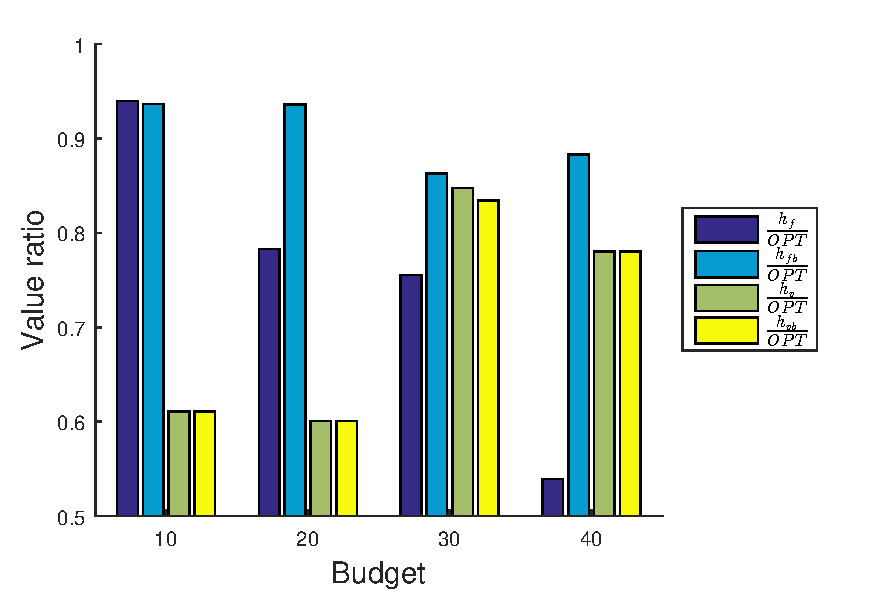
\includegraphics[width=0.46\textwidth]{images/bars_madagascar_value_ratio}\label{fig:previous_madagascar_utility}}
\subfigure[Time ratios]
 {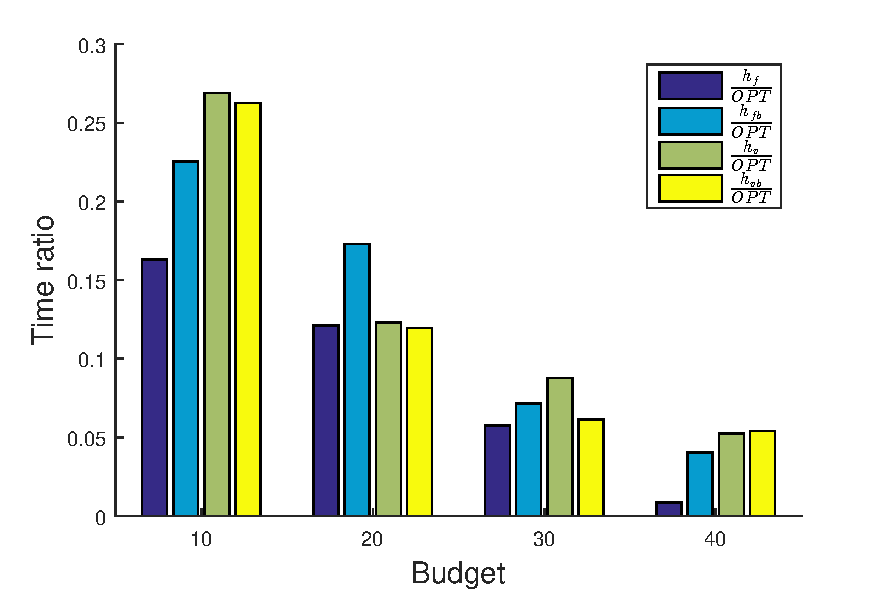
\includegraphics[width=0.46\textwidth]{images/bars_madagascar_time_ratio}\label{fig:previous_madagascar_time}}
\caption{Utility and time ratios of Algorithm~\ref{alg:approximation} w.r.t. FORTIFY on the Madagascar graph.}\label{fig:previous_madagascar}
\end{figure}

\textit{Results}. Differently from the synthetic instances, the results shown in Figure~\ref{fig:previous_madagascar} are apparently contradictory. Indeed, Figure~\ref{fig:previous_madagascar_utility} shows that, for low budgets, $h_v$ and $h_{vb}$ are performing much worse than $h_f, h_{fb}$. The rationale behind this trends is that $h_v$ and $h_{vb}$ form teams with just one type of resource, which results being the best in terms of utility and also the cheapest. As the budget increases, such behavior is mitigated and, adding diversity to the team, the performance improve, reaching also an approximation ratio close to 85\%. While the budget cannot help us in saying whether $h_v$ is always better than $h_{vb}$, it becomes very important when we take into account the features of the resources. In this case, including the budget results being the best behavior, which gives us an approximation ratio higher than 87\% even with a budget of 40. If we focus on Figure~\ref{fig:previous_madagascar_time}, we immediately notice that all the heuristics, independently of the budget, require always less than 30\% of the time employed by FORTIFY. Moreover, the higher the budget, the lower the time ratio. As for Figure~\ref{fig:previous_grid_time}, the apparently unusual trends of such ratio are due to the resolution of the problem for the chosen team.



%\textit{First pool}. Communal policemen and local volunteers conduct patrols in the forest. A typical patrol covers $20$ km in a day and patroller can conduct two types of patrols, a short patrol covering $2$ edges and a long patrol covering $3$ edges. Based on expert input, we assign the detection probability for communal police as $0.9$ for short patrols and $0.8$ for long patrols; and for volunteers, $0.7$ for short patrols and $0.6$ for long patrols. The lower probabilities for volunteers are because they must call backup for interdiction, which may allow the adversary to escape. Thus, in total we have $4$ resource types available $L = \{2,4,2,3\}, P = \{0.7,0.6,0.6,0.5\}$. The costs are proportional to the salaries patrollers receive for a day of patrolling $b = \{5,8,3,5\}$.
%\textit{Results}.

%\textit{Second pool}. Both policemen and volunteers can be enforced either with some sensors and devices, increasing its detection probability, or with vehicles, thus increasing its patrolling capacity, i.e., the number of edges that can be covedered. Thus, the new resources have the following features: $L = \{2,4,4,7,2,3,3,5\}, P = \{0.7,0.6,0.8,0.7,0.6,0.5,0.7,0.6\}, b = \{5,8,10,12,3,5,8,10\}$.
%\textit{Results}.

%Experiment: The runtime experiments are shown in Table 2 for increasing budgets. Data is averaged over 20 runs. FORTIFY can scale up to real world networks, able to handle both the large graph size and number of source and target nodes, even for large budgets. The value of performing this optimization is shown in Figure 7 with the solution quality (game value) on the y-axis and budget on the x-axis, where we compare the optimal game value to the average value achieved by randomly generated teams.

%We present four sets of experimental results: (1) We evaluate the scalability and runtime performance of FORTIFY on several classes of random graphs. We benchmark with a sequential search which sequentially evaluates enumerated teams with cost saturating the budget. (2) We also evaluate the impact of the initial compact layer on the runtime by comparing the runtimes of FORTIFY with and without the compact layer. (3) We investigate the benefit of optimizing team composition as well as the diversity of optimal teams and (4) we demonstrate that FORTIFY can scale up to the real world by testing performance on a case study of Madagascar using real graph data. All values are averaged over 20 trials.